Several examples of similiar desktop sized pinball machines exist. Apart from a few toys, most of the inspiration came from other enthusiasts who have constructed these machines themselves.
One throughouly explained example is by \textit{Element 14 Presents} on YouTube \cite{presents_2017}. Other videos used for inspiration includes \textit{Arduino Pinball Machine - 3d Printing \& Lasercutting} by Fluxwood \cite{fluxwood_2018}, \textit{Arduino Pinball - Target} by Functional Design\cite{functionaldesign_2017} and \textit{DIY Tabletop Pinball Machine - Making the cabinet \& decals} by The Practical Engineer \cite{engineer_2018}.
Although much of the bodywork and dimensions on the playfield came from reference images of full sized pinball machines - an example of one of those can be seen in figure \ref{fig:playfield_example}.

\begin{figure}
	\centering
	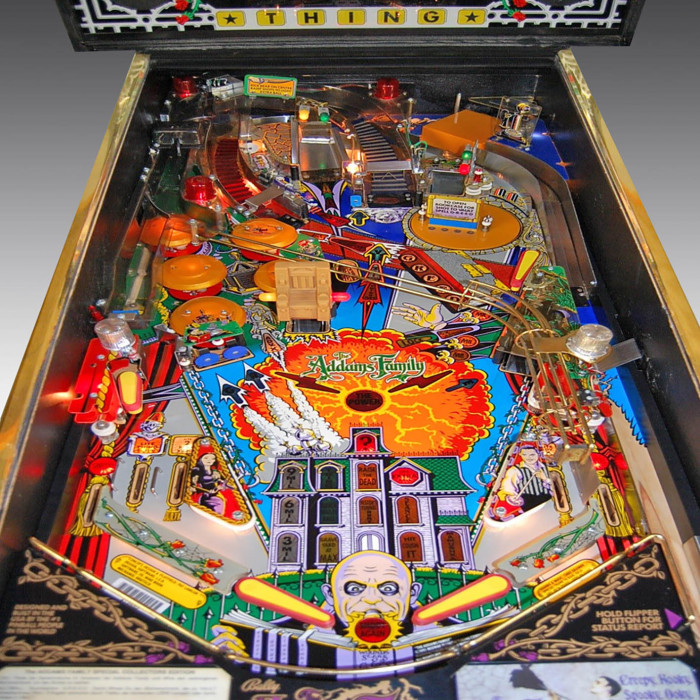
\includegraphics[scale=0.3]{img/example_playfield}
	\caption{Reference image of full sized pinball machine\cite{reference_picture}.}
	\label{fig:playfield_example}
\end{figure}